\documentclass[12pt]{article}
\usepackage{latexsym}
\usepackage{amssymb,amsmath}
\usepackage{float}
%%\usepackage[dvips]{graphicx}
\usepackage{graphicx}
%%\usepackage[dvips]{graphics}
\textwidth=6in \textheight=8.5in

\restylefloat{figure}

\begin{document}\begin{center}
CS 181\\
Problem Set 1
\end{center}

\begin{enumerate}

	\item 
		\begin{enumerate}
			\item
			\item
			\item
		\end{enumerate}

	\item
		\begin{enumerate}
			\item The average ten-fold cross-validation score for the non-noisy data is 0.87 while the score for noise data is 0.78.
			\item 
		\end{enumerate}


	\item
		\begin{enumerate}
			\item We are defining our information gain criterion to be the mutual information between an attribute and the label. However, we will modify all the calculated specific conditional entropies according to the weights of the examples. So instead of:
				\begin{center}
				$H(X|y) = \Sigma_x p(x|y) log_2 \frac{1}{p(x|y}$
				\end{center}
				We will be replacing the probability distribution $p$ with a weighted distribution based on the weights of the data. This way, data that is "more important" (the ones that tend to be predicted incorrectly) will be weighted more when the algorithm is trying to decide what attribute to split on. Attributes that split the more important data correctly will be favored over those that do not. For the example given where the label of the first example is $y_1 = 1$, etc, the weighted entropy of the set is 
				\begin{center}
				$0.5*log_{2}2 + 0.5*log_{2}2 = 1$.
				\end{center}
			\item
				\begin{enumerate}
					\item 
						Table of how the depth of the tree affects boosting\\\\
    							\begin{tabular}{|c|c|c|}
        							\hline
        							~            & 10 rounds & 20 rounds \\ \hline
        							maxDepth = 1 & 0.93      & 0.92      \\ 
        							maxDepth = 2 & 0.86      & 0.86      \\
        						\hline
    							\end{tabular}
						\\\\A larger maximum depth actually hurts the cross-validated test performance because when the individual trees are more complex, they are more susceptible to overfitting. This introduces trees with splits that are based more on noise than signal.
					\item 
						Boosting performs consistently worse on noisy data compared to non-noisy data no matter how many rounds (from 1 to 30) are performed. This is because the algorithm gives highers weights to data points that are predicted incorrectly. Therefore, if there are inconsistencies within the data, the algorithm will focus on the inconsistent data more than the rest of the data.
						\begin{figure}[H]
						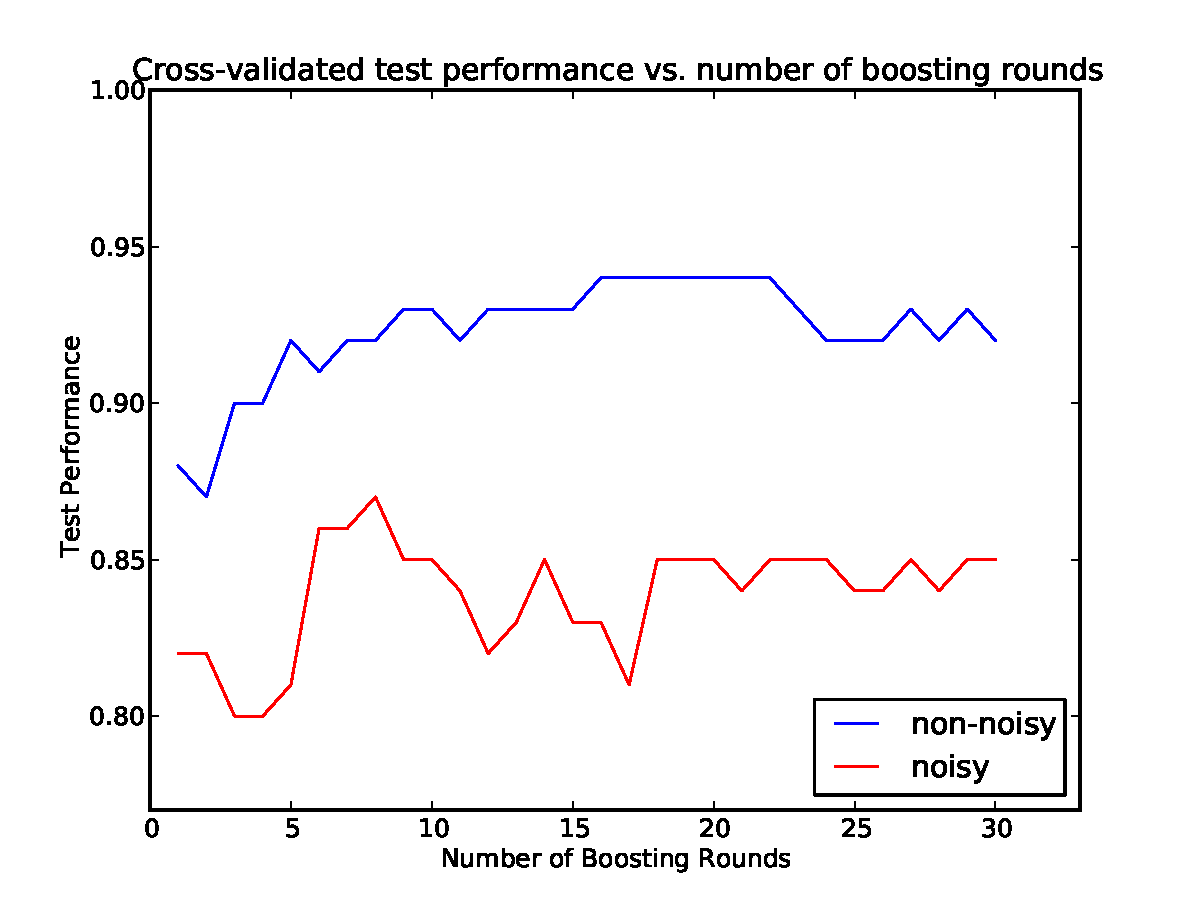
\includegraphics[width=150mm]{figure.pdf}
						\end{figure}
						
					\item 
					\item 
				\end{enumerate}
		\end{enumerate}

\end{enumerate}
\end{document}